\documentclass[11pt]{article}
\usepackage[a4paper,margin=2.1cm]{geometry}
\usepackage[T1]{fontenc}
\usepackage[utf8]{inputenc}
\usepackage{lmodern}
\usepackage{microtype}
\usepackage{graphicx}
\usepackage{booktabs}
\usepackage{longtable}
\usepackage{array}
\usepackage{tabularx}
\usepackage{multirow}
\usepackage{amsmath,amssymb}
\usepackage{siunitx}
\usepackage{xcolor}
\usepackage{listings}
\usepackage{caption}
\usepackage{subcaption}
\usepackage{enumitem}
\usepackage{fancyhdr}
\usepackage{hyperref}
\usepackage[numbers,sort&compress]{natbib}
\usepackage{url}
\usepackage{float}
\usepackage{placeins}
\usepackage{titlesec}
\usepackage{authblk}

\definecolor{codegray}{rgb}{0.96,0.96,0.96}
\definecolor{codegreen}{rgb}{0.1,0.45,0.1}
\definecolor{codeblue}{rgb}{0.1,0.2,0.65}
\lstdefinestyle{pythonstyle}{
  language=Python,
  backgroundcolor=\color{codegray},
  basicstyle=\ttfamily\small,
  keywordstyle=\color{codeblue}\bfseries,
  commentstyle=\color{codegreen},
  stringstyle=\color{purple},
  numbers=left,
  numberstyle=\tiny,
  stepnumber=1,
  numbersep=7pt,
  showstringspaces=false,
  breaklines=true,
  frame=single,
  columns=fullflexible,
  tabsize=4,
  captionpos=b
}
\lstset{style=pythonstyle}

\hypersetup{
  colorlinks=true,
  linkcolor=blue!55!black,
  citecolor=green!40!black,
  urlcolor=blue!65!black,
  pdftitle={Reverse Engineering and Reproducible Reconstruction of a Classical Fingerprint Feature-Extraction Laboratory Notebook},
  pdfauthor={Guillaume Harbonnier}
}

\pagestyle{fancy}
\fancyhf{}
\lhead{Fingerprint Feature Extraction Lab v1.0.0}
\rhead{Technical Report}
\cfoot{\thepage}
\setlength{\headheight}{14pt}
\setlist[itemize]{leftmargin=1.4em,itemsep=0.25em}
\setlist[enumerate]{leftmargin=1.6em,itemsep=0.25em}
\renewcommand{\arraystretch}{1.14}
\urlstyle{tt}
\setlength{\emergencystretch}{2em}

\title{\textbf{Reverse Engineering and Reproducible Reconstruction of a Classical Fingerprint Feature-Extraction Laboratory Notebook}\\[0.35em]
\large Minutiae, Skeleton Branches, Orientation Fields, and Core/Delta Candidates}
\author[1]{Guillaume Harbonnier}
\affil[1]{Independent technical research and biometric computer-vision laboratory}
\date{Version 1.0.0 -- 16 June 2026}

\begin{document}
\maketitle

\begin{abstract}
This report preserves and reconstructs an exploratory 483-cell fingerprint computer-vision notebook before its useful logic is lost inside duplicated experiments, state-dependent execution, contradictory comments, and an unverified biometric-template export branch. The reconstruction targets two outputs from one supplied fingerprint image: (i) ridge endings and bifurcations with skeleton-derived branch directions, and (ii) core/delta candidates with experimental local topology arms. The useful historical blocks are reorganized into a deterministic pipeline comprising grayscale loading, normalization, contrast-limited adaptive histogram equalization (CLAHE), foreground masking, structure-tensor orientation and coherence, Otsu ridge binarization, one-pixel skeletonization, conservative spur pruning, crossing-number candidates, multi-pixel junction consolidation, branch tracing, candidate quality gates, Poincare-index singularity detection, local position refinement, and auditable export. The strict one-image regression produces 33 accepted minutia candidates (31 endings and 2 bifurcations), two core candidates, and one delta candidate. These counts are not accuracy measurements because no expert ground truth or representative database is available. The report also isolates a major interoperability risk: the notebook's custom ISO/IEC 19794-2 writer mixes edition assumptions and validates itself with a parser built from the same private layout. It is therefore quarantined rather than represented as standard-conformant. The release includes the original notebook and PDF rendering, an all-cell audit, a cleaned executed notebook, reusable Python source, figures, CSV/JSON diagnostics, tests, LaTeX, the compiled PDF, and a GitHub-ready archive.
\end{abstract}

\noindent\textbf{Keywords:} fingerprint, minutiae, ridge ending, bifurcation, skeletonization, crossing number, orientation field, structure tensor, Poincare index, core, delta, BioCTS, reverse engineering, reproducible computer vision.

\section{Purpose and Scope}

The original laboratory notebook contains several genuinely useful classical-vision ideas, but they are distributed across experiments that were not designed to run sequentially. The most reliable skeleton appears near the bottom rather than near the first extraction branch. Cells marked informally with comments such as ``here yes,'' ``here no,'' and ``from there not'' encode important human judgments, but those judgments are not translated into a stable execution graph. Variables are overwritten, multiple definitions share the same function name, image conventions alternate between black-ridge and white-ridge skeletons, and OpenCV channel conversions are sometimes applied to already colorized images.

The objective of this work is preservation plus scientific reconstruction, not retrospective perfection. The deliverable answers four questions:

\begin{enumerate}
  \item Which historical blocks contain useful feature-extraction logic?
  \item In what order should those blocks be executed?
  \item Which assumptions and parameters control the resulting minutiae and singular points?
  \item Which branches must remain excluded because they are duplicated, broken, dependent on missing assets, or not independently validated?
\end{enumerate}

The scope is deliberately narrow. Only the supplied image \texttt{1.jpg} is used for the regression. No claim is made about false minutia rate, missed minutia rate, matcher accuracy, interoperability, template conformance, sensor robustness, or demographic/general population performance. The reconstructed output is best interpreted as a documented \emph{candidate extractor} and a platform for the next validation stage.

\section{Forensic Inventory of the Legacy Notebook}

\subsection{Primary artifacts}

The archival input consists of the following:

\begin{itemize}
  \item a 483-cell Jupyter notebook, \texttt{fingerprint\_lab.ipynb};
  \item a 208-page PDF rendering of that notebook;
  \item the test image \texttt{1.jpg};
  \item a first-acquisition image and two processed image variants;
  \item selected pasted outputs showing a good skeleton, minutiae, and core/delta overlays.
\end{itemize}

The PDF is useful because it preserves outputs that may no longer be reproducible from the current notebook state. For example, the early pages show the initial image and orientation field; later pages show a clean skeleton and a crossing-number output; the core/delta section shows two cyan candidate markers and one yellow candidate marker; and the final pasted output combines minutiae, singular points, and branches. The reconstruction preserves those images under \texttt{images/legacy/} rather than treating them as regenerated evidence.

\subsection{Cell-range disposition}

Table~\ref{tab:cellranges} gives the reverse-engineering decision for every major notebook region. A complete 483-row cell audit is distributed as \path{docs/legacy_cell_audit.csv} and \path{docs/legacy_cell_audit.md}.

\begin{table}[H]
\centering
\caption{Disposition of the legacy notebook by zero-based cell range.}
\label{tab:cellranges}
\small
\begin{tabularx}{\textwidth}{@{}p{1.45cm}p{2.65cm}X@{}}
\toprule
Cells & Decision & Reverse-engineering rationale \\
\midrule
0--7 & Keep/rewrite & Image loading, min--max normalization, CLAHE, and plotting form a useful start, but Colab/Drive paths are replaced with repository-relative paths. \\
8--20 & Keep/rewrite & The Sobel/structure-tensor orientation concept, axial smoothing, reliability mask, and visualization are useful. Duplicate masks, threshold ambiguity, and the repeated ``add $\pi/2$'' convention are consolidated. \\
21--26 & Split/rewrite & Skeleton, crossing number, mask resizing, border filtering, and drawing are mixed inside a large stateful block. They become separate tested functions. \\
27--42 & Keep/rewrite & Poincare-index core/delta logic is retained. Block-center quantization, duplicate detections, and grayscale/BGR failures are corrected or made explicit. \\
43--117 & Set aside & Predominantly repeated task prose, generated summaries, and duplicate code. Useful definitions already retained elsewhere are not executed twice. \\
118--260 & Quarantine & Custom ISO/FMR writer and self-parser. It mixes 2005/2011 assumptions and provides internal round-trip consistency rather than independent standard conformance. \\
261--289 & Keep/rewrite & Useful minutia filtering, local direction, and quality ideas are consolidated into branch tracing and explicit gates. \\
290--439 & Optional evaluation & Manual/expert-reference comparison depends on missing external annotation assets. It is an evaluation branch, not automatic extraction. \\
440--477 & Keep selectively & This late branch contains the visually best skeleton and useful enhancement/orientation experiments. Broken alternate ``thinning'' cells and environment mutations are excluded. \\
478--482 & Set aside & Drive-copy and session-export boilerplate is replaced by repository-relative output generation. \\
\bottomrule
\end{tabularx}
\end{table}

\subsection{Failure modes discovered by reverse engineering}

The most consequential defects are architectural rather than syntactic:

\begin{enumerate}
  \item \textbf{Execution-order inversion.} The best skeleton is produced after many downstream experiments that assume a skeleton already exists.
  \item \textbf{State ambiguity.} Names such as \texttt{img}, \texttt{mask}, \texttt{skeleton}, and \texttt{orientation} refer to different conventions at different times.
  \item \textbf{Axial versus directed angles.} A ridge orientation is axial modulo $\pi$, while a minutia branch is directed modulo $2\pi$. Adding $\pi/2$ can correct gradient-to-ridge conversion, but it cannot by itself choose a directed branch sense.
  \item \textbf{Skeleton polarity.} Some cells expect ridge pixels equal to 255, while others invert the skeleton for display and then reuse the displayed image as data.
  \item \textbf{Channel errors.} A drawing function unconditionally applies \texttt{cv2.cvtColor(..., COLOR\_GRAY2BGR)} even when the input is already BGR, causing the observed ``invalid number of channels'' exception.
  \item \textbf{Candidate inflation.} Crossing number on an unfiltered skeleton reports border endings, broken-ridge pairs, multi-pixel junction duplicates, and short-spur artifacts as minutiae.
  \item \textbf{Self-confirming serialization.} The binary writer and parser share the same assumptions. Their agreement cannot establish ISO/IEC conformance.
\end{enumerate}

\section{Scientific Processing Model}

The reconstructed pipeline follows the classical relationship between global ridge flow, local ridge topology, and singular points described in fingerprint literature \cite{hong1998enhancement,bazen2002directional,maltoni2009handbook}. Figure~\ref{fig:pipeline} shows the ordered stages.

\begin{figure}[H]
\centering
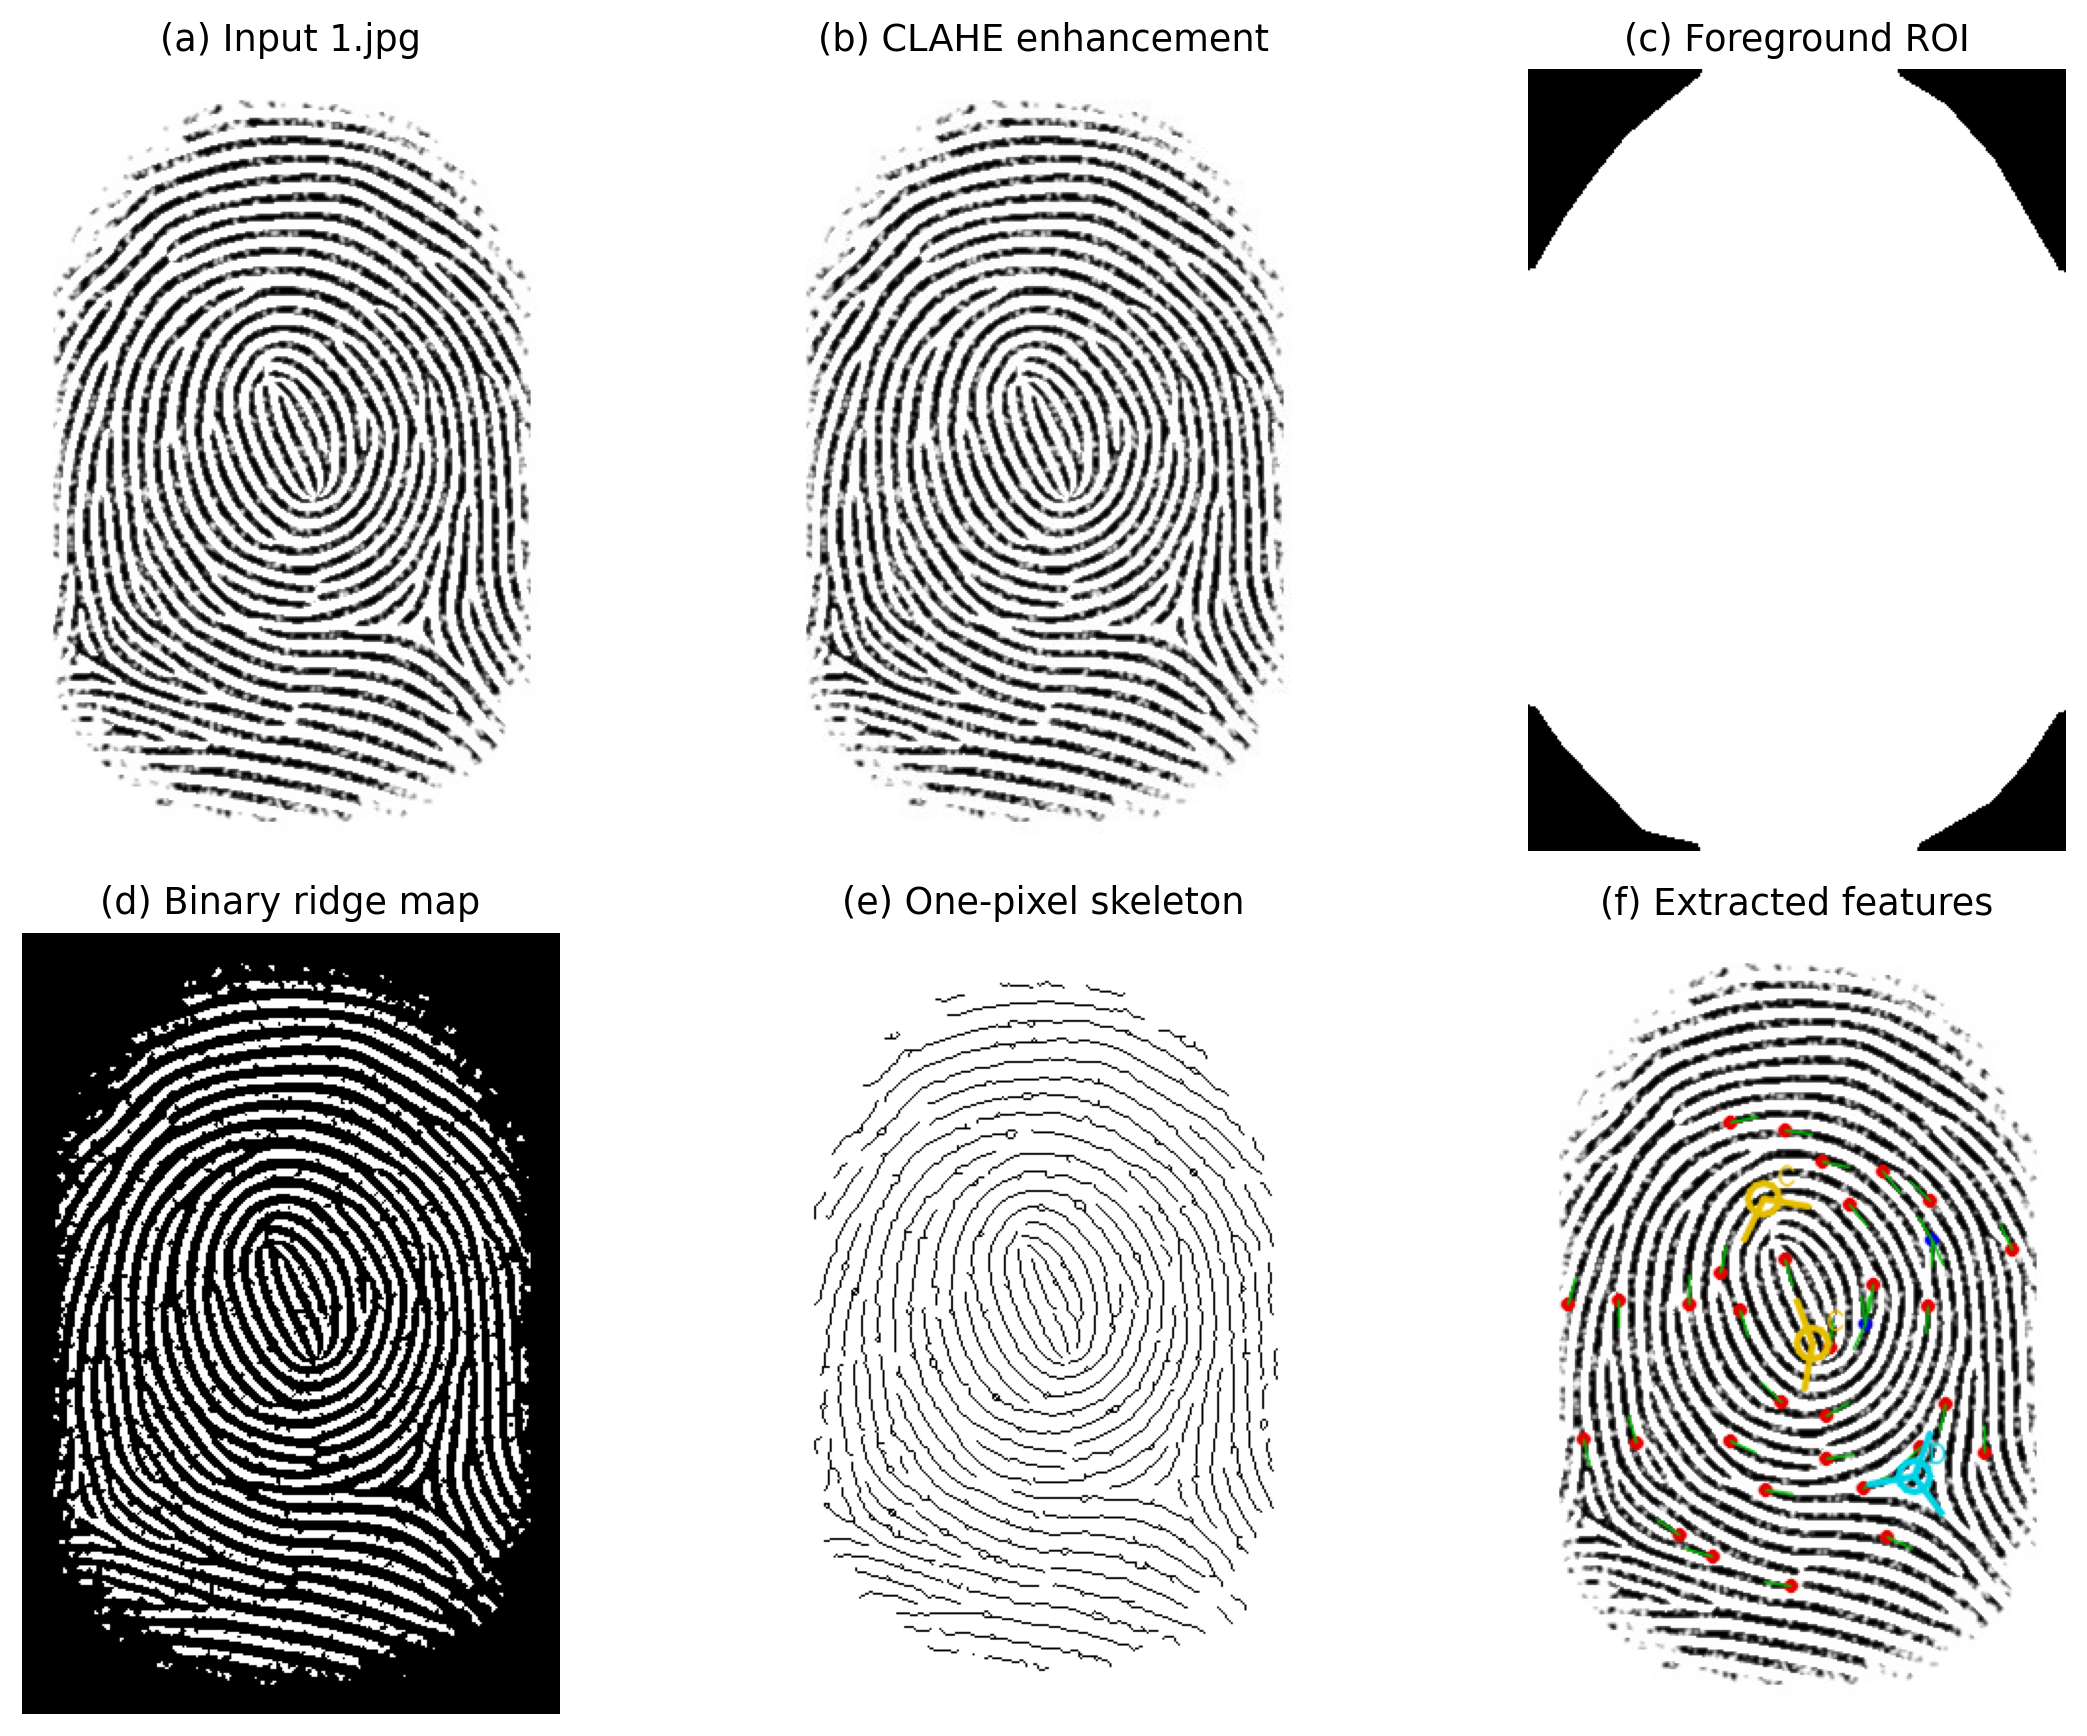
\includegraphics[width=0.96\textwidth]{../results/figure_pipeline_overview.png}
\caption{Canonical processing order on the single supplied image: input, CLAHE, ROI, binary ridges, skeleton, and extracted feature candidates.}
\label{fig:pipeline}
\end{figure}

\subsection{Input and photometric preprocessing}

Let $I:\Omega\rightarrow[0,255]$ be the grayscale image over pixel domain $\Omega$. Min--max normalization maps the observed range to $[0,255]$. CLAHE is then applied with a clip limit of 2.0 and an $8\times8$ tile grid. This preserves the useful first notebook branch without implying that CLAHE is universally optimal for fingerprint enhancement.

The supplied image already has high ridge/valley contrast. Therefore, the final strict branch uses Otsu thresholding after CLAHE rather than the notebook's incomplete pixel-wise Gabor loop. Gabor enhancement is well established for orientation- and frequency-adaptive fingerprint enhancement \cite{hong1998enhancement}, but a correct implementation requires a locally estimated ridge frequency, stable padding, and orientation/frequency quality control. The exploratory cells did not yet provide those conditions consistently.

\subsection{Foreground region of interest}

The current ROI is intentionally image-specific. The white background is thresholded, dark ridge fragments are joined by morphological closing and dilation, the largest component is retained, and its convex hull is filled. A second, eroded mask defines a conservative interior in which minutiae may be accepted.

This distinction is important:

\begin{itemize}
  \item the \emph{foreground mask} supports orientation estimation and ridge binarization;
  \item the \emph{inner mask} prevents border cuts from being interpreted as ridge endings.
\end{itemize}

This is not a general fingerprint segmentation algorithm. A future dataset version should replace the white-background heuristic with a quality-aware segmentation model and test it across sensors, crops, pressure levels, and dry/wet impressions.

\subsection{Structure-tensor orientation and coherence}

Sobel derivatives $G_x$ and $G_y$ are computed. Over a local support, the structure tensor is

\begin{equation}
J = \begin{bmatrix}
J_{xx} & J_{xy}\\
J_{xy} & J_{yy}
\end{bmatrix}
= \begin{bmatrix}
\mathcal{G}_{\sigma}*(G_x^2) & \mathcal{G}_{\sigma}*(G_xG_y)\\
\mathcal{G}_{\sigma}*(G_xG_y) & \mathcal{G}_{\sigma}*(G_y^2)
\end{bmatrix},
\end{equation}
where $\mathcal{G}_{\sigma}$ is Gaussian smoothing. The principal gradient-axis estimate is

\begin{equation}
\theta_g = \frac{1}{2}\operatorname{atan2}(2J_{xy},J_{xx}-J_{yy}).
\end{equation}

The ridge tangent is perpendicular to the gradient axis:

\begin{equation}
\theta_r = \left(\theta_g + \frac{\pi}{2}\right) \bmod \pi.
\end{equation}

A coherence proxy is

\begin{equation}
\kappa = \frac{\sqrt{(J_{xx}-J_{yy})^2 + 4J_{xy}^2}}{J_{xx}+J_{yy}+\epsilon}.
\end{equation}

This follows the averaged-square-gradient/PCA interpretation analyzed by Bazen and Gerez \cite{bazen2002directional}. Coherence is used as a reliability gate, not as a calibrated biometric quality value.

Because $\theta_r$ and $\theta_r+\pi$ represent the same ridge axis, direct averaging of angles is invalid near the wrap boundary. Smoothing is therefore performed in double-angle space:

\begin{equation}
\bar{\theta}_r = \frac{1}{2}\operatorname{atan2}\left(
\mathcal{G}_{\sigma}*\sin 2\theta_r,
\mathcal{G}_{\sigma}*\cos 2\theta_r
\right).
\end{equation}

The implementation creates both a $16\times16$ block field for audit/visualization and a dense field for singularity refinement. Figure~\ref{fig:orientation} shows the field and coherence.

\begin{figure}[H]
\centering
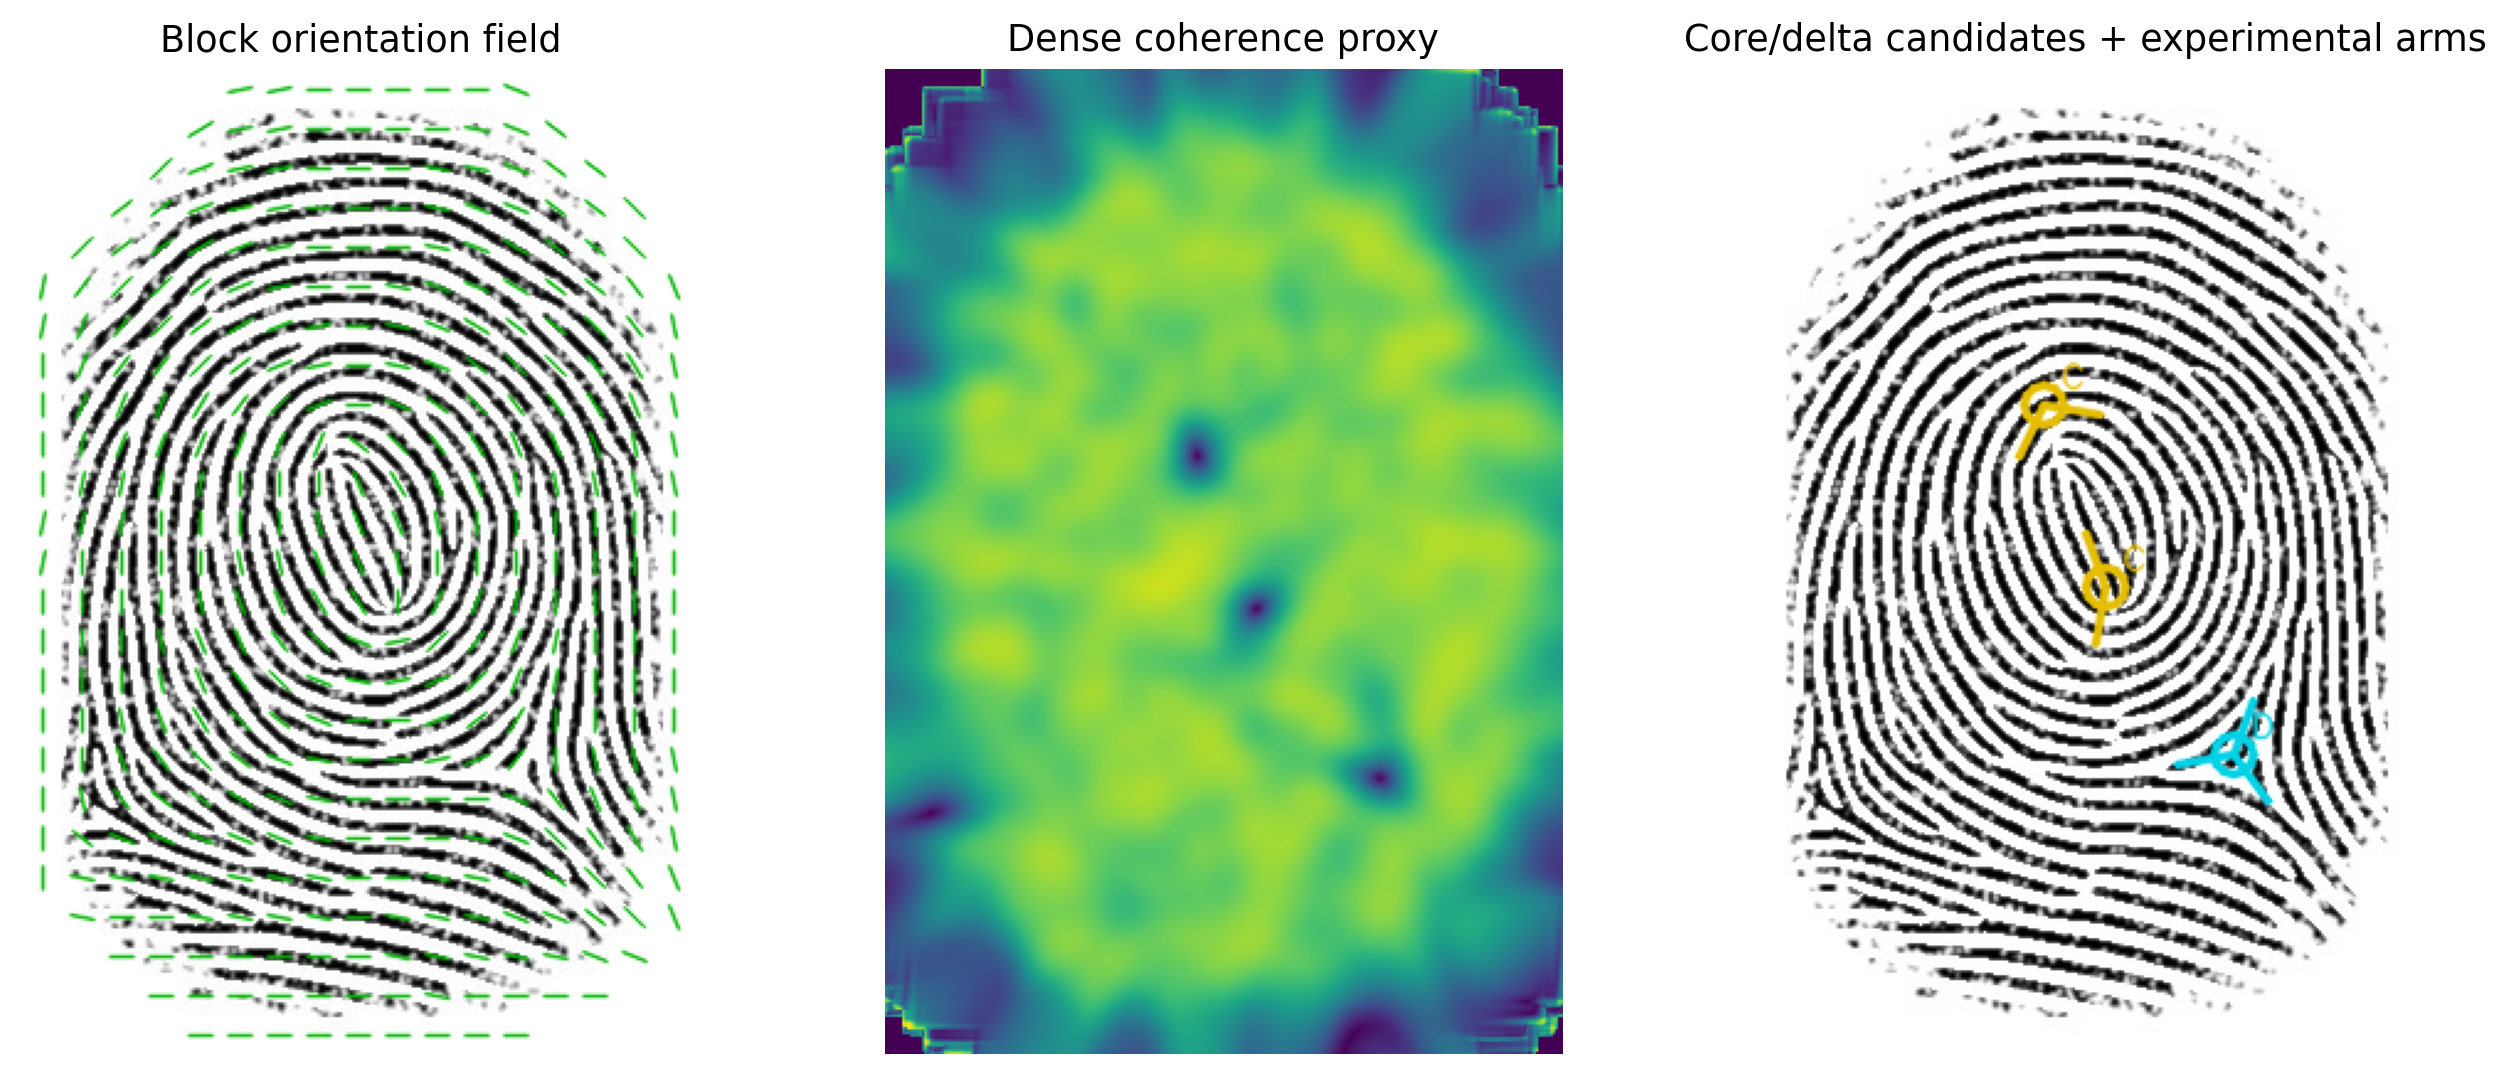
\includegraphics[width=0.96\textwidth]{../results/figure_singularity_diagnostics.png}
\caption{Orientation and singularity diagnostics. The coherence image is a structure-tensor reliability proxy. Core/delta arm rays are experimental topology cues.}
\label{fig:orientation}
\end{figure}

\subsection{Ridge binarization and skeletonization}

Global Otsu inversion creates a binary ridge map inside the ROI. Tiny foreground components are removed. A one-pixel skeleton is then produced using \texttt{skimage.morphology.skeletonize}. Skeletonization is a topological reduction problem; classic thinning literature emphasizes connectivity preservation and the risk of spurious branches \cite{lam1992thinning,zhang1984fast}. OpenCV also provides a Zhang--Suen thinning operation in \texttt{ximgproc} \cite{opencvthinning}; the reconstructed code uses scikit-image for a fixed, directly tested dependency.

Only short endpoint-to-junction spurs are pruned. Aggressive thinning cleanup can erase real endings, so the chosen maximum length is five skeleton steps. This is a conservative engineering choice rather than an optimized parameter.

\subsection{Crossing-number minutia candidates}

For a skeleton pixel $p$ with ordered binary neighbors $P_1,\ldots,P_8$ around the 8-neighborhood, the crossing number is

\begin{equation}
\operatorname{CN}(p) = \frac{1}{2}\sum_{i=1}^{8}\left|P_i-P_{i+1}\right|,
\qquad P_9=P_1.
\end{equation}

The standard interpretation is CN$=1$ for an ending and CN$=3$ for a bifurcation \cite{thai2002preprocessing}. This produces \emph{raw candidates}, not valid minutiae. On the current skeleton, 436 candidate pixels are observed before clustering and filtering.

\subsection{Multi-pixel junction consolidation}

A real bifurcation rarely becomes one perfect skeleton pixel. A small junction may contain several adjacent pixels with CN$=3$, and direct drawing would place multiple minutiae around one physical event. The reconstruction therefore:

\begin{enumerate}
  \item groups nearby candidate pixels of the same type;
  \item chooses a representative center;
  \item removes/collapses the local candidate zone;
  \item identifies connected skeleton components that leave that zone;
  \item traces one physical arm per component.
\end{enumerate}

This graph interpretation is the central improvement over assigning a direction from the block orientation field alone.

\subsection{Directed branch orientation}

The ridge field is axial modulo $\pi$, but a branch starting at a minutia is directed modulo $2\pi$. For a traced path ending at $(x_e,y_e)$ from candidate $(x_m,y_m)$, the branch angle is

\begin{equation}
\phi = \operatorname{atan2}(y_e-y_m, x_e-x_m) \bmod 2\pi.
\end{equation}

An ending must yield exactly one sufficiently long arm. A bifurcation must yield exactly three. This avoids the legacy shortcut that flips a block orientation based on a single local grayscale gradient and then reverses it for bifurcations. That shortcut can orient a line visually, but it does not reconstruct three distinct branches.

\subsection{Quality gates and artifact suppression}

A candidate is accepted only if it satisfies all of the following:

\begin{enumerate}
  \item it lies within the eroded interior mask and at least 38 pixels from that mask boundary;
  \item local coherence is at least 0.40;
  \item its reconstructed arm count is one or three, according to candidate type;
  \item every arm traces at least 15 skeleton steps;
  \item it is at least 20 pixels from an already accepted candidate;
  \item it is not one of two short, facing endings across a gap that is likely a broken ridge.
\end{enumerate}

A non-standard quality proxy combines coherence and normalized minimum branch length. It is exported explicitly as \texttt{quality\_proxy}; it is not encoded as an ISO quality score.

\subsection{Poincare-index core and delta candidates}

The orientation field is an axial field, so differences are wrapped into $[-\pi/2,\pi/2]$. Around a closed eight-block ring, the Poincare sum is

\begin{equation}
P = \sum_{k=1}^{8}\operatorname{wrap}_{[-\pi/2,\pi/2]}
(\theta_{k+1}-\theta_k), \qquad \theta_9=\theta_1.
\end{equation}

Positive and negative singular rotations generate core and delta candidates, respectively. The implementation uses thresholds above $+\pi/2$ and below $-\pi/2$, clusters adjacent candidate blocks, then searches a pixel neighborhood with a denser circular Poincare loop.

The Poincare method is computationally simple and widely used, but it is sensitive to local orientation noise, coarse block placement, duplicate candidates, and crop effects \cite{bazen2002directional,ohtsuka2007core}. This explains the user's correct observation: the type can appear plausible while the exact location remains displaced.

\subsection{Experimental singularity arms}

Core/delta arms are visualized from peaks in radial/tangent alignment on a ring around the refined singularity. Three separated peaks are retained for a delta; two cues are retained for a core. These rays are useful for diagnosing the field but have not been validated against expert singularity directions. They must not be confused with minutia branch directions, which are traced directly on the skeleton.

\section{Canonical Implementation and Execution Order}

\subsection{Single entry point}

The canonical implementation is \path{src/fingerprint_pipeline.py}. The function \path{run_pipeline} is the only ordered entry point. Listing~\ref{lst:entry} shows the architecture in abbreviated form.

\begin{lstlisting}[caption={Canonical orchestration. The complete source is included in the repository.},label={lst:entry}]
def run_pipeline(image_path, cfg=None):
    cfg = cfg or PipelineConfig()
    original = load_grayscale(image_path)
    normalized, enhanced = normalize_and_clahe(original, cfg)
    roi_mask, inner_roi_mask = compute_roi_mask(original, cfg)
    theta_b, coh_b, theta_dense, coh_dense = estimate_orientation_fields(
        enhanced, roi_mask, cfg
    )
    binary, skeleton, skeleton_diag = binarize_and_skeletonize(
        enhanced, roi_mask, cfg
    )
    minutiae, minutiae_diag = extract_and_filter_minutiae(
        skeleton, inner_roi_mask, coh_dense, cfg
    )
    singular_points, singular_diag = detect_singular_points(
        theta_b, coh_b, theta_dense, coh_dense, inner_roi_mask, cfg
    )
    return PipelineResult(...)
\end{lstlisting}

\subsection{Line-by-line function map}

Table~\ref{tab:linewalk} links source ranges to their role. The repository contains a longer prose walkthrough in \path{docs/source_code_walkthrough.md}.

\small
\begin{longtable}{@{}p{1.35cm}p{5.25cm}p{8.05cm}@{}}
\caption{Near-line-level map of the canonical 938-line module.}\label{tab:linewalk}\\
\toprule
Lines & Function/block & Detailed role \\
\midrule
\endfirsthead
\toprule
Lines & Function/block & Detailed role \\
\midrule
\endhead
1--23 & Module contract/imports & Declares the research-only boundary and imports fixed numerical/image dependencies. \\
24--49 & \path{PipelineConfig} & Centralizes every threshold and eliminates hidden notebook state. \\
50--75 & \path{Minutia}, \path{SingularPoint} & Defines coordinates, semantic type, branch angles/lengths, coherence, ROI distance, and quality proxy. \\
76--98 & \path{PipelineResult} & Retains all intermediate arrays for audit and visualization. \\
99--107 & \path{load_grayscale} & Reads a single-channel image and fails early on missing/invalid input. \\
108--117 & \path{normalize_and_clahe} & Reconstructs the first useful preprocessing cells with explicit parameters. \\
118--126 & \path{largest_component} & Uses connected components to suppress unrelated foreground islands. \\
127--159 & \path{compute_roi_mask} & Thresholds the white background, joins ridges, fills a convex hull, and erodes a safe interior. \\
160--173 & \path{_smooth_axial_field} & Smooths $\cos 2\theta$ and $\sin 2\theta$ with optional mask normalization. \\
174--230 & \path{estimate_orientation_fields} & Computes Sobel tensors, dense/block ridge tangents, coherence, ROI-valid blocks, and axial smoothing. \\
231--268 & \path{binarize_and_skeletonize} & Applies Otsu inversion, ROI masking, optional morphology, small-object removal, skeletonization, and pruning. \\
269--287 & Neighborhood and CN & Enumerates 8-connected ridge pixels and computes crossing number. \\
288--324 & Spur pruning & Repeatedly follows endpoints toward junctions and removes only paths no longer than the configured maximum. \\
325--430 & Branch tracing helpers & Traces smooth graph paths and reconstructs physical arms around multi-pixel junctions. \\
431--490 & Cluster-aware branch descriptors & Removes a candidate cluster zone, finds outgoing components, estimates geodesic lengths, and returns directed arm angles. \\
491--525 & Raw candidates/clustering & Finds CN$=1$/CN$=3$ pixels and groups nearby candidates of the same type. \\
526--566 & Broken-ridge pair suppression & Removes short pairs of endings whose missing directions face each other across a gap. \\
567--636 & Minutia quality gates & Applies interior, coherence, arm count/length, separation, and pair-suppression rules; exports diagnostics. \\
637--687 & Axial Poincare utilities & Wraps orientation increments, computes block/dense loop indices, and clusters spatial candidates. \\
688--728 & Singularity arm cues & Scores radial/tangent alignment and chooses separated visualization peaks. \\
729--808 & Singularity detection/refinement & Detects block candidates, clusters them, searches pixel neighborhoods, and emits core/delta records. \\
809--842 & \path{run_pipeline} & Executes all stages once and merges configuration plus stage diagnostics. \\
843--898 & Drawing & Handles grayscale/BGR safely and draws orientation, minutia arms, and singularity cues. \\
899--938 & Table/JSON export & Writes explicit units and lists to CSV and diagnostic metadata to JSON. \\
\bottomrule
\end{longtable}
\normalsize

\subsection{Critical implementation excerpts}

Listing~\ref{lst:axial} shows why orientation smoothing must use double angles.

\begin{lstlisting}[caption={Mask-normalized axial smoothing.},label={lst:axial}]
def _smooth_axial_field(theta, sigma, mask=None):
    c = np.cos(2.0 * theta)
    s = np.sin(2.0 * theta)
    if mask is None:
        c_s = gaussian_filter(c, sigma=sigma)
        s_s = gaussian_filter(s, sigma=sigma)
    else:
        m = mask.astype(float)
        den = gaussian_filter(m, sigma=sigma) + 1e-8
        c_s = gaussian_filter(c * m, sigma=sigma) / den
        s_s = gaussian_filter(s * m, sigma=sigma) / den
    return 0.5 * np.arctan2(s_s, c_s)
\end{lstlisting}

Listing~\ref{lst:cn} shows the crossing-number kernel. It is intentionally small; most of the work lies in what happens \emph{after} the raw candidate is found.

\begin{lstlisting}[caption={Crossing number on the ordered 8-neighborhood.},label={lst:cn}]
def crossing_number_at(skeleton_bool, y, x):
    vals = []
    for dy, dx in OFFSETS_8:
        yy, xx = y + dy, x + dx
        vals.append(1 if in_bounds_and_ridge(yy, xx) else 0)
    return sum(abs(vals[i] - vals[(i + 1) % 8])
               for i in range(8)) // 2
\end{lstlisting}

Listing~\ref{lst:gates} summarizes the candidate acceptance logic. The exact implementation records a rejection count for every gate.

\begin{lstlisting}[caption={Conservative candidate gates, abbreviated.},label={lst:gates}]
if inner_roi_mask[y, x] == 0 or roi_dist[y, x] < min_roi_distance:
    reject("outside_inner_roi")
if coherence[y, x] < min_coherence:
    reject("low_coherence")
if len(branch_angles) != expected_branch_count(kind):
    reject("invalid_branch_count")
if min(branch_lengths) < min_branch_length:
    reject("short_branch")
if near_an_accepted_candidate(x, y):
    reject("near_duplicate")
\end{lstlisting}

\section{Parameters, Libraries, and Reproducibility}

\subsection{Frozen parameters}

Table~\ref{tab:params} records the strict configuration. These values are frozen for the one-image regression; they are not fitted or validated on a dataset.

\footnotesize
\begin{longtable}{@{}p{6.05cm}p{1.85cm}p{6.85cm}@{}}
\caption{Configuration in release 1.0.0.}\label{tab:params}\\
\toprule
Parameter & Value & Interpretation \\
\midrule
\endfirsthead
\toprule
Parameter & Value & Interpretation \\
\midrule
\endhead
\path{block_size} & 16 px & Orientation block size and initial singularity grid. \\
\path{clahe_clip_limit} & 2.0 & Local histogram clipping. \\
\path{clahe_grid} & $8\times8$ & CLAHE tile grid. \\
\path{orientation_smooth_sigma_blocks} & 1.0 & Gaussian smoothing in block space on double-angle components. \\
\path{roi_dark_threshold} & 248 & White-background separation threshold. \\
\path{roi_close_size} & 19 px & Joins ridge fragments for the foreground envelope. \\
\path{roi_erode_px} & 25 px & Defines conservative interior. \\
\path{min_component_size} & 24 px & Removes small binary foreground components. \\
\path{prune_length} & 5 steps & Maximum short endpoint-to-junction spur removed. \\
\path{minutia_roi_distance} & 38 px & Minimum distance inside the eroded ROI. \\
\path{minutia_min_coherence} & 0.40 & Tensor-coherence gate. \\
\path{minutia_min_separation} & 20 px & Greedy inter-candidate separation. \\
\path{branch_trace_length} & 18 steps & Maximum local arm tracing length. \\
\path{branch_min_length} & 15 steps & Minimum accepted arm length. \\
\path{broken_ridge_pair_max_gap} & 24 px & Maximum gap for facing-ending suppression. \\
\path{broken_ridge_pair_angle_tolerance} & 35 deg & Directional tolerance for gap suppression. \\
\path{singular_search_radius} & 10 px & Dense local refinement radius. \\
\path{singular_ring_radius} & 10 px & Ring radius for experimental topology arms. \\
\path{singular_min_coherence} & 0.12 & Minimum block coherence for singularity candidates. \\
\bottomrule
\end{longtable}
\normalsize

\subsection{Software environment}

The executed release used Python 3.13 with the packages shown in Table~\ref{tab:versions}. The repository includes both \texttt{requirements.txt} and \texttt{environment.yml}.

\begin{table}[H]
\centering
\caption{Executed software versions.}
\label{tab:versions}
\begin{tabular}{@{}ll@{}}
\toprule
Library & Version \\
\midrule
OpenCV / opencv-contrib-python & 4.13.0 \\
NumPy & 2.3.5 \\
SciPy & 1.17.0 \\
scikit-image & 0.26.0 \\
Matplotlib & 3.10.8 \\
Pandas & 2.2.3 \\
nbformat & 5.10.4 \\
\bottomrule
\end{tabular}
\end{table}

\subsection{Reproduction commands}

\begin{lstlisting}[language=bash,caption={Repository-level reproduction.}]
python -m venv .venv
# activate the environment, then:
pip install -r requirements.txt
python src/run_experiment.py
pytest -q
jupyter lab notebooks/fingerprint_feature_extraction_reconstructed.ipynb
\end{lstlisting}

The executed notebook contains no Drive mount and no mid-run package mutation. It imports the reusable module from \texttt{src/}, displays each major stage, prints diagnostics, and reads the exported CSV tables.

\section{One-Image Results}

\subsection{Stage diagnostics}

The image shape is $400\times275$ pixels. Otsu selects threshold 153. The binary ridge map contains 30,061 foreground pixels. The final skeleton contains 7,761 ridge pixels; 75 short-spur pixels are removed in one pruning iteration.

Raw crossing number finds 436 candidate pixels, consolidated into 330 local candidate clusters. The strict gates accept 41 candidates before broken-ridge-pair suppression; eight facing endpoints are then removed, leaving 33 candidates.

\begin{table}[H]
\centering
\caption{Strict one-image regression diagnostics.}
\label{tab:results}
\begin{tabular}{@{}lr@{}}
\toprule
Diagnostic & Value \\
\midrule
Raw crossing-number pixels & 436 \\
Candidate clusters & 330 \\
Rejected: outside conservative interior & 129 \\
Rejected: low coherence & 5 \\
Rejected: invalid arm count & 94 \\
Rejected: short arm & 32 \\
Rejected: near duplicate & 29 \\
Accepted before broken-ridge suppression & 41 \\
Suppressed facing endings & 8 \\
Final minutia candidates & 33 \\
Ridge endings & 31 \\
Bifurcations & 2 \\
Block singularity candidates & 12 \\
Singularity clusters & 3 \\
Core candidates & 2 \\
Delta candidates & 1 \\
\bottomrule
\end{tabular}
\end{table}

The rejection counts should not be read as errors against ground truth. They are deterministic gate outcomes.

\subsection{Minutiae and branches}

Figure~\ref{fig:minutiae} compares the skeleton with accepted candidates and their overlay on the original image. Red circles indicate endings, blue circles bifurcations, and green rays the skeleton-derived directed arms.

\begin{figure}[H]
\centering
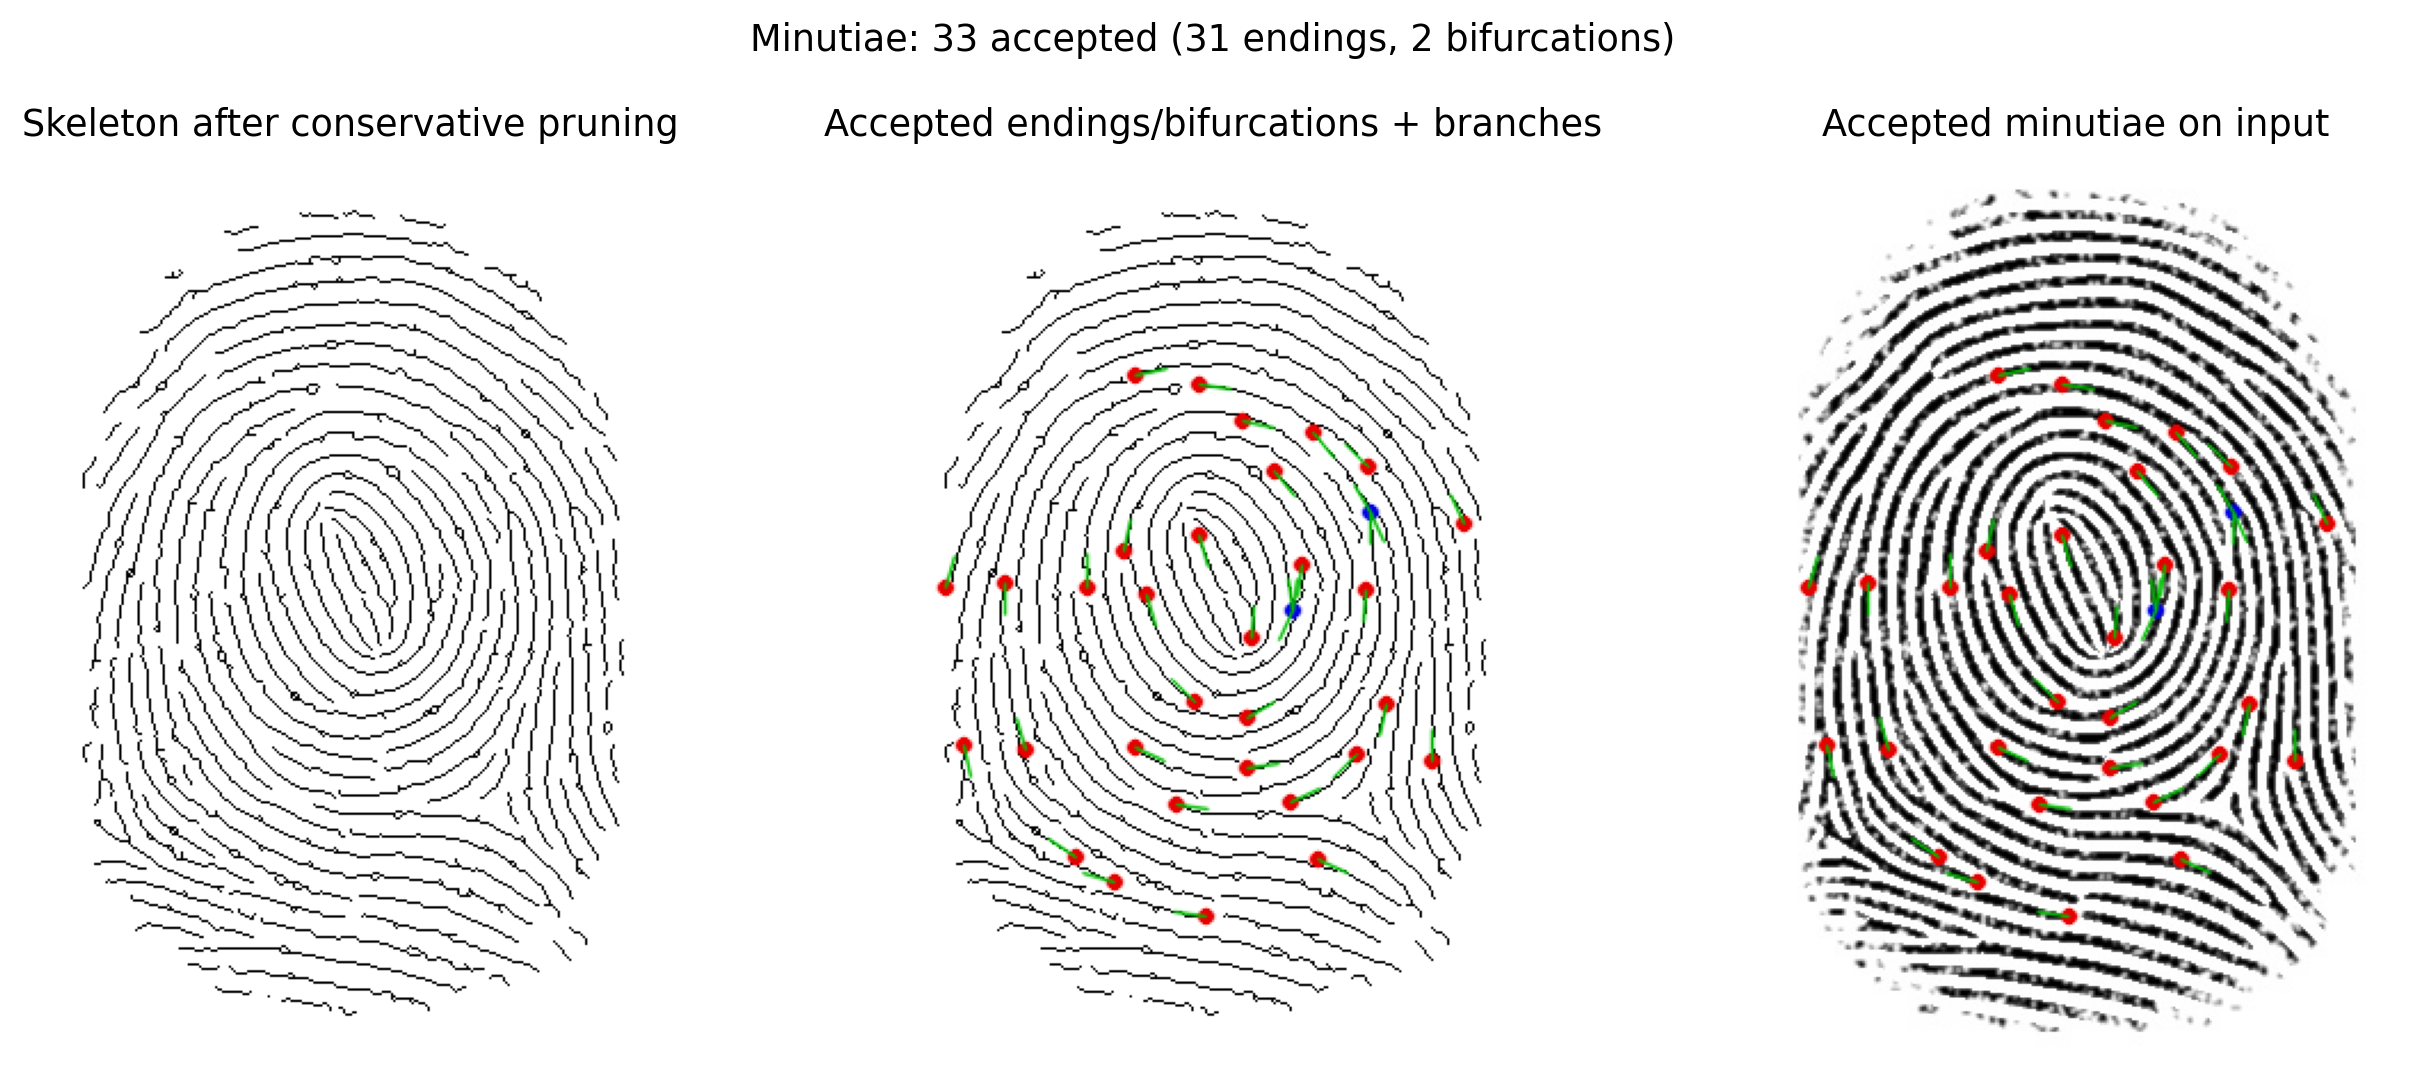
\includegraphics[width=0.98\textwidth]{../results/figure_minutiae_diagnostics.png}
\caption{Strict accepted minutiae. The reduction relative to the legacy visualization results from explicit interior, coherence, arm-count, arm-length, separation, and broken-ridge rules.}
\label{fig:minutiae}
\end{figure}

The strict branch deliberately produces few bifurcations. This is preferable to presenting noisy CN$=3$ pixels as valid junctions, but it may also reject real bifurcations when one arm is broken or too short. A future expert-annotated evaluation should therefore compare at least two operating points:

\begin{itemize}
  \item a permissive candidate set for high recall;
  \item a strict branch-valid set for higher apparent precision.
\end{itemize}

\subsection{Core/delta candidates}

The current output contains cores at approximately $(120,136)$ and $(145,210)$, and a delta at approximately $(197,278)$, in top-left image coordinates. Their Poincare indices are approximately $+\pi$, $+\pi$, and $-\pi$ respectively. Figure~\ref{fig:combined} shows the combined view.

\begin{figure}[H]
\centering
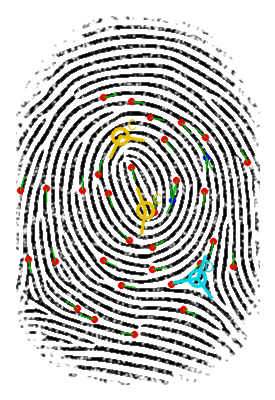
\includegraphics[height=0.64\textheight]{../results/11_combined_features.png}
\caption{Combined strict feature output. Red: ending. Blue: bifurcation. Yellow: core candidate. Cyan: delta candidate. Green/minor colored rays: local branch or topology cues.}
\label{fig:combined}
\end{figure}

The types are visually plausible for the whorl-like flow, but the exact positions remain uncertain. The block Poincare stage initially localizes topology only to a $16$-pixel grid; dense refinement reduces but does not remove sensitivity to smoothing, ring radius, and crop. The user-observed delta arms are partly plausible, while one branch is weak; the current report therefore labels all singularity arms experimental.

\subsection{Legacy versus reconstruction}

Figure~\ref{fig:legacy} separates archival evidence from regenerated output. The legacy view contains many more candidates and appears visually rich, but its exact variable state cannot be reconstructed confidently. The new view is less dense and fully traceable.

\begin{figure}[H]
\centering
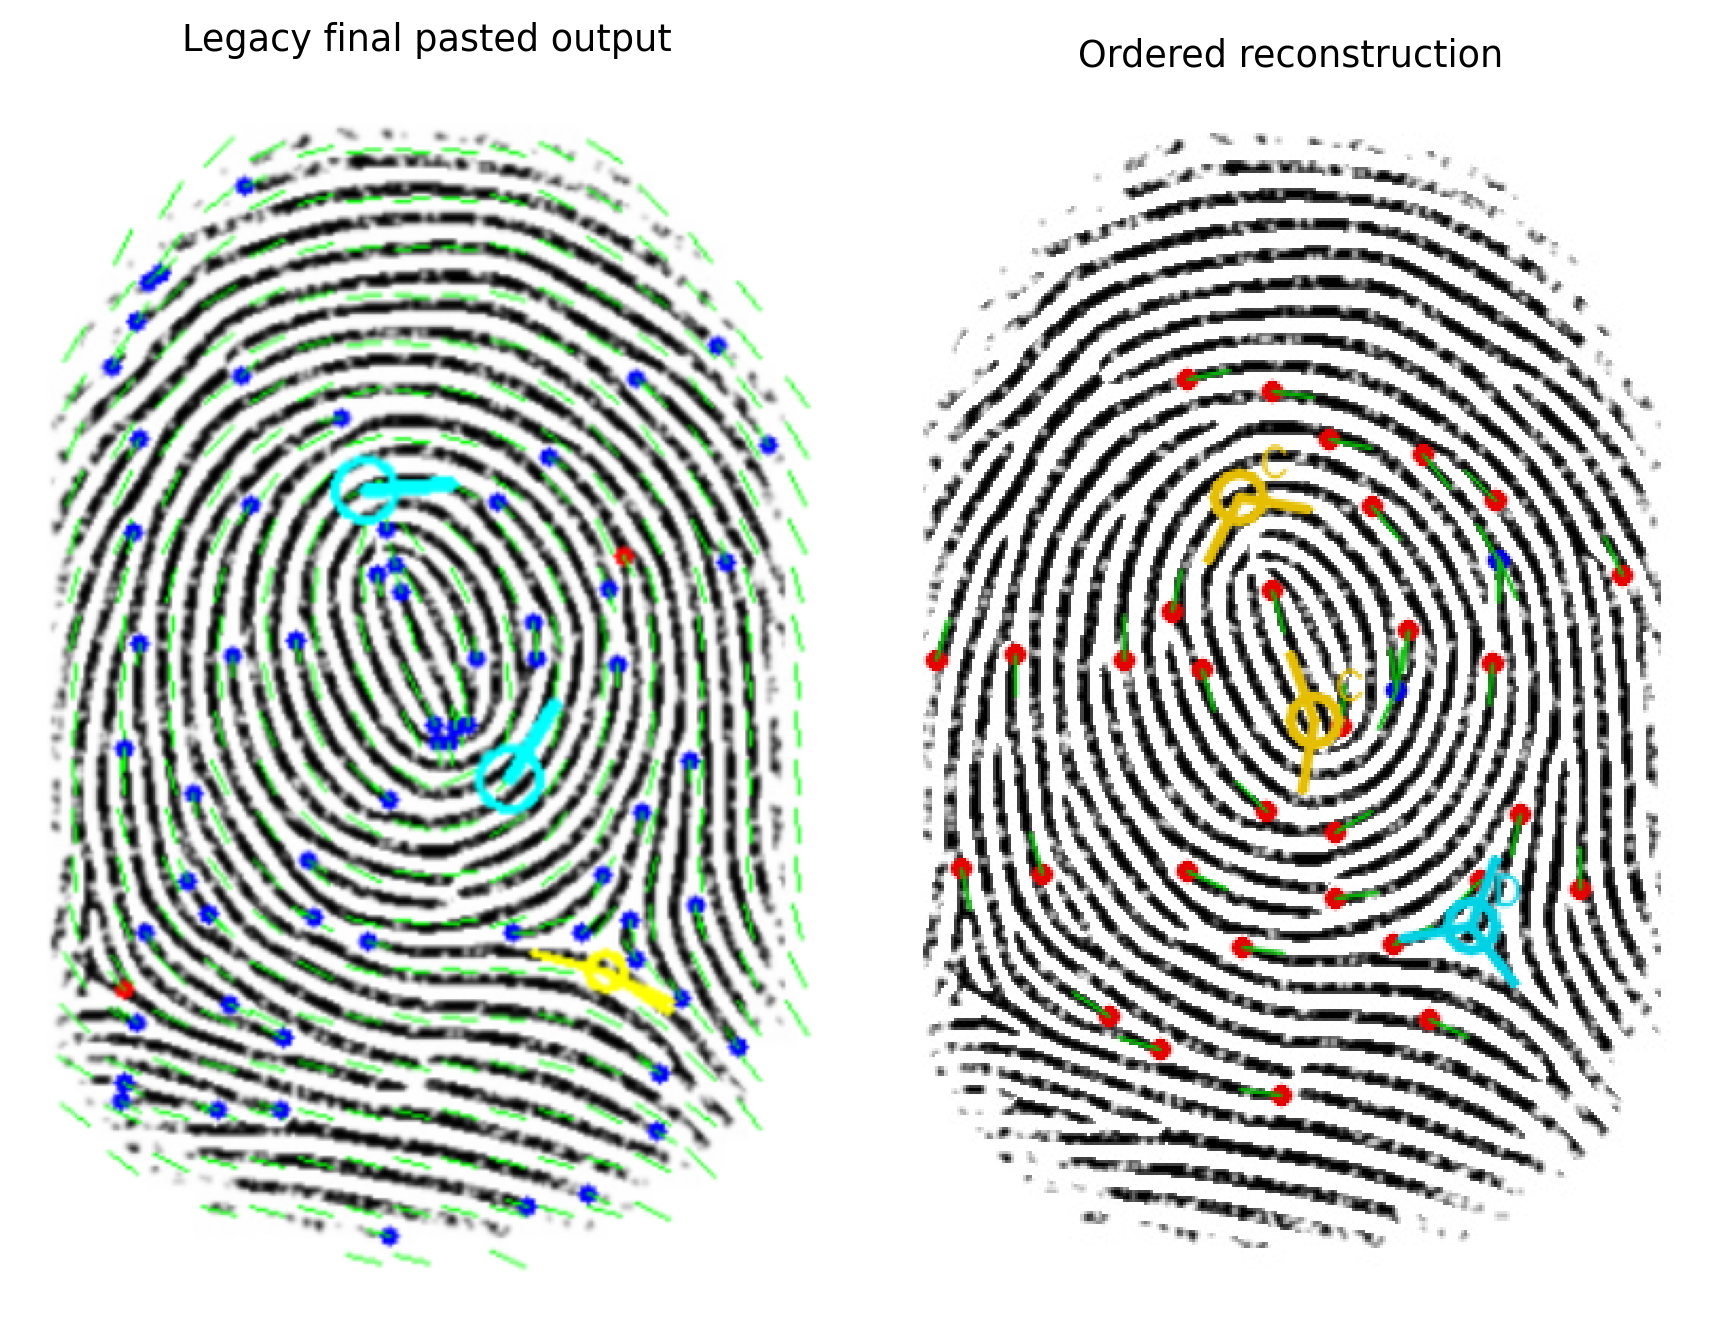
\includegraphics[width=0.88\textwidth]{../results/figure_legacy_vs_reconstructed.png}
\caption{Left: preserved legacy final pasted output. Right: deterministic ordered reconstruction. The comparison is qualitative because the legacy state and expert ground truth are unavailable.}
\label{fig:legacy}
\end{figure}

\section{Why Some Directions Were Wrong in the Legacy Output}

The historical observation ``position and orientation axis look correct, but some minutiae point in the wrong direction'' has a precise cause. A structure-tensor ridge field returns an \emph{axis}:

\begin{equation}
\theta \equiv \theta+\pi.
\end{equation}

An ending, however, needs an outgoing or incoming \emph{vector}. A local image gradient can help pick one of the two directions, but it is unreliable exactly at a ridge termination because local intensity derivatives are affected by the termination geometry, thresholding, and neighboring valleys. For a bifurcation, one vector is insufficient in principle because three arms must be represented.

The reconstructed method derives the directed angle from the skeleton path. This improves semantic consistency but remains dependent on skeleton quality. If a ridge is broken, the path can stop early; if a junction is thick or contains a loop, component separation can merge or duplicate arms. Therefore the code exports both angles and traced lengths so suspect directions can be audited.

\section{ISO/IEC 19794-2 and BioCTS: Quarantine Analysis}

\subsection{What the standard family actually covers}

ISO/IEC 19794-2:2005 defines minutiae-based fingerprint data elements, record-based exchange, normal and compact match-on-card formats, and optional extended data including ridge counts and core/delta locations \cite{iso1979422005}. The 2011 edition likewise defines fundamental minutiae data and three interchange/storage formats, with optional extended core/delta-related data \cite{iso1979422011}.

This already shows why a simplified header followed by repeated six-byte private records is not sufficient evidence of conformance. A conformant encoder must choose the correct edition and format, obey all mandatory header and representation rules, handle finger-view metadata and extension blocks correctly, and implement the standard's exact coordinate, angle, type, quality, length, and reserved-field semantics.

\subsection{Why the notebook's writer is not accepted}

The historical writer branch exhibits the following red flags:

\begin{enumerate}
  \item its prose requests the 2005 standard but later changes the magic/version assumptions toward 2011;
  \item the proposed header is assembled from an inferred private \texttt{struct} layout rather than a fully cited clause-by-clause schema;
  \item the minutia count is changed from one byte to two because a run produced 1,106 raw candidates, but a field cannot be changed merely because the current data does not fit;
  \item angle and quality ranges are alternately described as degrees, 0--179, 0--255, 0--100, and 0--254;
  \item the parser validates the same layout generated by the writer, so successful parsing is circular;
  \item the output contains 1,106 ``minutiae,'' largely before robust candidate filtering, which is itself a warning that the exported semantic content is not meaningful.
\end{enumerate}

The reconstructed repository therefore does \textbf{not} generate an FMR/FPT file. The legacy branch remains available for forensic review but outside the executable path.

\subsection{Correct validation path}

NIST's BioCTS distribution includes conformance test suites for both ISO/IEC 19794-2:2005 and ISO/IEC 19794-2:2011 binary finger-minutiae data \cite{nistbiocts2026}. NIST also describes BiomDI as partially supporting biometric records including ISO/IEC 19794-2/19794-4, while warning that support varies by utility \cite{nistbiomdi}. A defensible implementation plan is:

\begin{enumerate}
  \item obtain and use the licensed official edition and any applicable corrigenda/amendments;
  \item implement a clause-mapped encoder and an independent decoder;
  \item add golden byte vectors and negative tests for lengths, reserved fields, view counts, extension lengths, coordinate limits, and angle encoding;
  \item validate with BioCTS for the exact selected edition/profile;
  \item cross-check with a second independent implementation where available;
  \item only then label generated files as standard-conformant.
\end{enumerate}

The report intentionally does not reproduce proprietary clause text or byte tables from the copyrighted ISO publication.

\section{Error Analysis and Limitations}

\subsection{No ground truth}

The largest limitation is not algorithmic: there is no expert minutia annotation file aligned to \texttt{1.jpg}. Visual plausibility cannot measure precision or recall. The manual-reference branch in the legacy notebook suggests that such a comparison was contemplated, but its Drive-resident images/annotations are absent from the uploaded package.

\subsection{Single-image parameter coupling}

Every threshold can overfit the supplied impression. The white-background ROI, 38-pixel interior distance, 20-pixel separation, and 15-step arm length are especially coupled to the image scale. Resolution metadata is not independently known from the JPEG. Consequently, pixel distances must not be interpreted as physical ridge distances.

\subsection{Binarization and skeleton topology}

Otsu works well visually on this high-contrast image. It may fail on latent, dry, wet, blurred, compressed, low-contrast, or unevenly illuminated impressions. Broken ridges create paired false endings; merged ridges create false bifurcations; skeletonization can move junction centers by several pixels.

\subsection{Core/delta ambiguity}

Singularity detection depends on orientation accuracy. The Poincare method uses local angular circulation and can produce location error, core/delta confusion, or duplicate detections under noise \cite{ohtsuka2007core}. A whorl may have two cores and two deltas, but crop and segmentation can hide or distort one singularity. This report does not infer a final Henry class from the three detected candidates.

\subsection{No matcher or template-quality study}

The project stops at feature candidates. It does not align two impressions, estimate elastic deformation, compare minutia sets, or produce FAR/FRR/DET results. It also does not claim NFIQ-style quality, ISO quality, or matcher utility.

\section{Validation Roadmap}

A reviewer-defensible next version should proceed in stages.

\subsection{Stage A: expert annotation on the current image}

Create an annotation JSON with image hash, coordinate convention, ending/bifurcation type, directed branch angles, core/delta locations, and uncertainty radius. Evaluate candidate matching under a distance/angle tolerance rather than exact pixel equality. Report strict and permissive operating points.

\subsection{Stage B: multi-impression same-finger consistency}

Use multiple impressions of the same fingers. After registration, measure location repeatability, type consistency, angle error, and feature survival. This distinguishes extractor instability from identity variation.

\subsection{Stage C: representative public benchmarks}

Evaluate on a dataset with licensing compatible with repository release. Separate threshold selection from test evaluation. Report per-sensor and per-quality strata, not one aggregate number.

\subsection{Stage D: component ablation}

Ablate CLAHE, ROI erosion, coherence gate, spur pruning, branch-count gate, broken-ridge suppression, and dense singularity refinement. Measure which components reduce false candidates and which suppress valid minutiae.

\subsection{Stage E: standards branch}

Create a separate \texttt{iso-fmr} branch only after feature semantics are stable. The encoder must be clause-mapped, version-specific, independently parsed, and BioCTS-tested. It should not be merged merely because a private parser round-trips the file.

\section{Repository Deliverables}

\small
\begin{longtable}{@{}p{7.15cm}p{7.65cm}@{}}
\caption{Release artifact catalogue.}\label{tab:artifacts}\\
\toprule
Artifact & Purpose \\
\midrule
\endfirsthead
\toprule
Artifact & Purpose \\
\midrule
\endhead
\path{legacy/fingerprint_lab_legacy_unordered.ipynb} & Exact historical notebook archive. \\
\path{legacy/fingerprint_lab_legacy_render.pdf} & 208-page historical rendering preserving outputs and errors. \\
\path{notebooks/fingerprint_feature_extraction_reconstructed.ipynb} & Clean, ordered, executed notebook using repository-relative paths. \\
\path{src/fingerprint_pipeline.py} & Reusable 938-line implementation with typed data structures and explicit configuration. \\
\path{src/run_experiment.py} & Generates all figures, PNG stages, tables, and diagnostics. \\
\path{docs/legacy_cell_audit.csv} & Machine-readable disposition of all 483 cells. \\
\path{docs/legacy_cell_audit.md} & Human-readable all-cell audit. \\
\path{docs/block_execution_order.md} & Exact canonical order and excluded branches. \\
\path{docs/source_code_walkthrough.md} & Function/line-range explanation. \\
\path{results/minutiae.csv} & Coordinates, type, directed branch angles, branch lengths, coherence, ROI distance, and quality proxy. \\
\path{results/singular_points.csv} & Core/delta candidates, Poincare index, experimental arms, and coherence. \\
\path{results/diagnostics.json} & Frozen parameters and all stage/candidate counts. \\
\path{tests/test_pipeline.py} & Shape, binary skeleton, nonempty bounded output, branch-cardinality, and coordinate regression tests. \\
\path{paper/main.tex}, \path{paper/references.bib}, PDF & Full technical report and citations. \\
\bottomrule
\end{longtable}
\normalsize

\section{Conclusion}

The notebook does contain a coherent classical fingerprint feature-extraction experiment, but that experiment was hidden by order inversion, variable reuse, duplicate generated prose, mixed image conventions, and an unsafe standards branch. Reverse engineering recovers a clear core:

\begin{quote}
foreground and contrast $\rightarrow$ orientation/coherence $\rightarrow$ ridge map $\rightarrow$ skeleton topology $\rightarrow$ branch-valid minutiae $\rightarrow$ Poincare singularity candidates $\rightarrow$ auditable outputs.
\end{quote}

The reconstructed run preserves what worked---especially the late good skeleton, crossing-number concept, orientation field, and Poincare candidates---while refusing to convert visual plausibility into unsupported claims. Minutia directions now come from traced skeleton arms. Core/delta positions are refined but still explicitly uncertain. The ISO/FMR writer is preserved as history and quarantined until a version-specific, independently tested implementation exists.

The result is not a finished fingerprint extractor. It is a reproducible scientific baseline from which real validation can begin without losing the original exploration.

\clearpage
\appendix

\section{Detailed Canonical Run Order}

\begin{enumerate}
  \item Set a fixed environment; do not install or uninstall OpenCV mid-notebook.
  \item Resolve repository root and load \texttt{images/input/1.jpg} in grayscale.
  \item Assert nonempty two-dimensional input.
  \item Min--max normalize the grayscale range.
  \item Apply CLAHE with frozen clip limit and tile grid.
  \item Threshold dark pixels against the white background.
  \item Morphologically join fragments for the foreground envelope.
  \item Retain the largest component and fill its convex hull.
  \item Erode the foreground to construct a conservative minutia interior.
  \item Compute Sobel $x/y$ gradients on the enhanced image.
  \item Build dense structure-tensor components.
  \item Convert gradient principal axis to ridge tangent by $+\pi/2$.
  \item Compute dense coherence.
  \item Smooth ridge orientation in double-angle space under the ROI.
  \item Aggregate a separate 16-pixel block orientation/coherence field.
  \item Apply Otsu inverse threshold and mask outside the ROI.
  \item Remove small foreground objects.
  \item Skeletonize to one-pixel ridges.
  \item Prune short endpoint-to-junction spurs only.
  \item Compute crossing number for every skeleton pixel.
  \item Label CN$=1$ as raw ending and CN$=3$ as raw bifurcation.
  \item Cluster adjacent candidates of the same type.
  \item Collapse each candidate cluster/junction zone.
  \item Find outgoing connected skeleton arms.
  \item Trace arms and calculate directed angles and geodesic lengths.
  \item Apply inner-ROI distance and coherence gates.
  \item Require exact physical arm cardinality: one or three.
  \item Require minimum arm length and candidate separation.
  \item Suppress short facing endpoint pairs across likely ridge gaps.
  \item Export strict minutia records.
  \item Compute block Poincare index on valid interior blocks.
  \item Cluster core/delta candidate blocks.
  \item Refine each cluster by dense local circular Poincare search.
  \item Estimate experimental singularity topology rays.
  \item Export singularity records, figures, CSV, and JSON diagnostics.
\end{enumerate}

\section{Blocks Explicitly Excluded from the Default Run}

\begin{itemize}
  \item all repeated task prose and duplicated summaries;
  \item all cells that depend on notebook state without defining their inputs;
  \item manual expert-reference comparison without supplied annotations;
  \item package uninstall/reinstall cells;
  \item alternate erosion/contour operations labeled as thinning without topology verification;
  \item the custom 2005/2011 FMR serialization and self-parser;
  \item Google Drive copy/list operations;
  \item claims that file length equality or local parser equality proves biometric conformance.
\end{itemize}

\section{Interpretation of Exported Fields}

\subsection{Minutiae CSV}

\begin{description}
  \item[\texttt{x,y}] top-left-origin pixel coordinates in the supplied image.
  \item[\texttt{kind}] \texttt{ending} or \texttt{bifurcation}, based initially on crossing number and retained only after arm validation.
  \item[\texttt{orientation\_rad}] first directed branch angle for convenience; for bifurcations the complete list must be used.
  \item[\texttt{branch\_angles\_rad}] one or three directed angles in $[0,2\pi)$ derived from skeleton geometry.
  \item[\texttt{branch\_lengths\_px}] traced geodesic lengths in skeleton steps/pixels.
  \item[\texttt{coherence}] local structure-tensor coherence proxy.
  \item[\texttt{roi\_distance\_px}] distance-transform value inside the conservative inner mask.
  \item[\texttt{quality\_proxy}] internal $[0,1]$ combination of coherence and minimum branch length; not a standardized quality.
\end{description}

\subsection{Singular points CSV}

\begin{description}
  \item[\texttt{x,y}] refined pixel candidate location.
  \item[\texttt{kind}] \texttt{core} or \texttt{delta} from Poincare sign.
  \item[\texttt{poincare\_index\_rad}] dense local loop sum after axial wrapping.
  \item[\texttt{branch\_angles\_rad}] experimental ring-alignment topology cues.
  \item[\texttt{coherence}] dense orientation coherence at the refined point.
\end{description}

\section{Regression-Test Interpretation}

The tests intentionally avoid asserting exact biometric correctness. They verify software invariants:

\begin{itemize}
  \item all raster dimensions match;
  \item skeleton values are binary;
  \item the skeleton is nontrivial;
  \item the one-image output remains nonempty and bounded;
  \item at least one ending, bifurcation, core, and delta are present;
  \item coordinates remain within image bounds;
  \item endings have one stored arm and bifurcations have three;
  \item quality proxies stay inside $[0,1]$.
\end{itemize}

Exact counts are recorded in diagnostics but not hard-coded as scientific truth. Small algorithmic improvements should be allowed to change them while still satisfying invariants.

\section{Reviewer Checklist for a Future Dataset Release}

\begin{enumerate}
  \item Are train/tuning/test images separated before parameter selection?
  \item Is image resolution known and are pixel thresholds normalized physically?
  \item Are expert annotations created independently by at least two examiners or adjudicated?
  \item Are ending/bifurcation type, position tolerance, and angle convention documented?
  \item Are strict and permissive operating points both reported?
  \item Are failures stratified by sensor, quality, crop, and fingerprint class?
  \item Is skeleton topology inspected for broken/merged ridges?
  \item Are core/delta duplicates, missing singularities, and positional error reported separately?
  \item Does every standards claim identify exact edition, amendment, record format, and test suite?
  \item Are all figures regenerable from a clean environment and repository-relative paths?
\end{enumerate}

\begin{thebibliography}{99}

\bibitem[Hong et~al.(1998)Hong, Wan, and Jain]{hong1998enhancement}
L. Hong, Y. Wan, and A. K. Jain.
\newblock Fingerprint image enhancement: Algorithm and performance evaluation.
\newblock \emph{IEEE Transactions on Pattern Analysis and Machine Intelligence}, 20(8):777--789, 1998.
\newblock doi: \href{https://doi.org/10.1109/34.709565}{10.1109/34.709565}.

\bibitem[Bazen and Gerez(2002)]{bazen2002directional}
A. M. Bazen and S. H. Gerez.
\newblock Systematic methods for the computation of the directional fields and singular points of fingerprints.
\newblock \emph{IEEE Transactions on Pattern Analysis and Machine Intelligence}, 24(7):905--919, 2002.
\newblock doi: \href{https://doi.org/10.1109/TPAMI.2002.1017618}{10.1109/TPAMI.2002.1017618}.

\bibitem[Lam et~al.(1992)Lam, Lee, and Suen]{lam1992thinning}
L. Lam, S.-W. Lee, and C. Y. Suen.
\newblock Thinning methodologies---a comprehensive survey.
\newblock \emph{IEEE Transactions on Pattern Analysis and Machine Intelligence}, 14(9):869--885, 1992.
\newblock doi: \href{https://doi.org/10.1109/34.161346}{10.1109/34.161346}.

\bibitem[Zhang and Suen(1984)]{zhang1984fast}
T. Y. Zhang and C. Y. Suen.
\newblock A fast parallel algorithm for thinning digital patterns.
\newblock \emph{Communications of the ACM}, 27(3):236--239, 1984.
\newblock doi: \href{https://doi.org/10.1145/357994.358023}{10.1145/357994.358023}.

\bibitem[Thai(2002)]{thai2002preprocessing}
R. Thai.
\newblock Fingerprint image enhancement and minutiae extraction.
\newblock In \emph{CISST 2002 International Conference}, pages 742--745, 2002.

\bibitem[Ohtsuka et~al.(2007)Ohtsuka, Watanabe, and Aoki]{ohtsuka2007core}
T. Ohtsuka, D. Watanabe, and H. Aoki.
\newblock Fingerprint core and delta detection by candidate analysis.
\newblock In \emph{IAPR Conference on Machine Vision Applications}, pages 130--133, 2007.

\bibitem[Maltoni et~al.(2009)Maltoni, Maio, Jain, and Prabhakar]{maltoni2009handbook}
D. Maltoni, D. Maio, A. K. Jain, and S. Prabhakar.
\newblock \emph{Handbook of Fingerprint Recognition}.
\newblock Springer, second edition, 2009.

\bibitem[ISO/IEC(2005)]{iso1979422005}
ISO/IEC.
\newblock ISO/IEC 19794-2:2005, biometric data interchange formats---Part 2: Finger minutiae data.
\newblock Official catalogue page: \url{https://www.iso.org/standard/38746.html}, 2005.

\bibitem[ISO/IEC(2011)]{iso1979422011}
ISO/IEC.
\newblock ISO/IEC 19794-2:2011, biometric data interchange formats---Part 2: Finger minutiae data.
\newblock Official catalogue page: \url{https://www.iso.org/standard/50864.html}, 2011.

\bibitem[NIST(2026a)]{nistbiocts2026}
National Institute of Standards and Technology.
\newblock BioCTS for ISO/IEC biometric data interchange format standards and selected PIV profiles.
\newblock \url{https://www.nist.gov/services-resources/software/biometric-testing-software/biometric-conformance-test-software-biocts-0}, 2026.

\bibitem[NIST(2026b)]{nistbiomdi}
National Institute of Standards and Technology.
\newblock BiomDI---software tools supporting standard biometric data interchange formats.
\newblock \url{https://www.nist.gov/services-resources/software/biomdi-software-tools-supporting-standard-biometric-data-interchange}, 2026.

\bibitem[OpenCV(2026)]{opencvthinning}
OpenCV.
\newblock Extended image processing: thinning.
\newblock \url{https://docs.opencv.org/4.x/df/d2d/group__ximgproc.html}, accessed 2026-06-16.

\end{thebibliography}

\end{document}
